\documentclass[12pt,preprint]{aastex}

% has to be before amssymb it seems
\usepackage{color,hyperref}
\definecolor{linkcolor}{rgb}{0,0,0.5}
\hypersetup{colorlinks=true,linkcolor=linkcolor,citecolor=linkcolor,
            filecolor=linkcolor,urlcolor=linkcolor}

\usepackage{url}
\usepackage{algorithmic,algorithm}
\usepackage{amssymb,amsmath}

\usepackage{listings}
\definecolor{lbcolor}{rgb}{0.9,0.9,0.9}
\lstset{language=Python,
        basicstyle=\footnotesize\ttfamily,
        showspaces=false,
        showstringspaces=false,
        tabsize=2,
        breaklines=false,
        breakatwhitespace=true,
        identifierstyle=\ttfamily,
        keywordstyle=\bfseries\color[rgb]{0.133,0.545,0.133},
        commentstyle=\color[rgb]{0.133,0.545,0.133},
        stringstyle=\color[rgb]{0.627,0.126,0.941},
    }

\newcommand{\project}[1]{{\sffamily #1}}
\newcommand{\Python}{\project{Python}}
\newcommand{\numpy}{\project{numpy}}
\newcommand{\license}{MIT License}

\newcommand{\foreign}[1]{\emph{#1}}
\newcommand{\etal}{\foreign{et\,al.}}
\newcommand{\etc}{\foreign{etc.}}

\newcommand{\Fig}[1]{Figure~\ref{fig:#1}}
\newcommand{\fig}[1]{\Fig{#1}}
\newcommand{\figlabel}[1]{\label{fig:#1}}
\newcommand{\Tab}[1]{Table~\ref{tab:#1}}
\newcommand{\tab}[1]{\Tab{#1}}
\newcommand{\tablabel}[1]{\label{tab:#1}}
\newcommand{\Eq}[1]{Equation~(\ref{eq:#1})}
\newcommand{\eq}[1]{\Eq{#1}}
\newcommand{\eqlabel}[1]{\label{eq:#1}}
\newcommand{\Sect}[1]{Section~\ref{sect:#1}}
\newcommand{\sect}[1]{\Sect{#1}}
\newcommand{\App}[1]{Appendix~\ref{sect:#1}}
\newcommand{\app}[1]{\App{#1}}
\newcommand{\sectlabel}[1]{\label{sect:#1}}
\newcommand{\Algo}[1]{Algorithm~\ref{algo:#1}}
\newcommand{\algo}[1]{\Algo{#1}}
\newcommand{\algolabel}[1]{\label{algo:#1}}

% math symbols
\newcommand{\dd}{\mathrm{d}}
\newcommand{\bvec}[1]{\boldsymbol{#1}}
\newcommand{\unit}[1]{\mathrm{#1}}

\begin{document}

\title{Bart:\ Fast and flexible modeling of exoplanet transits}

\newcommand{\nyu}{2}
\newcommand{\mpia}{3}
\author{%
    Daniel~Foreman-Mackey\altaffilmark{1,\nyu},
    Patrick Cooper\altaffilmark{\nyu}, and
    David~W.~Hogg\altaffilmark{\nyu,\mpia}
}
\altaffiltext{1}{To whom correspondence should be addressed:
                        \url{danfm@nyu.edu}}
\altaffiltext{\nyu}{Center for Cosmology and Particle Physics,
                        Department of Physics, New York University,
                        4 Washington Place, New York, NY, 10003, USA}
\altaffiltext{\mpia}{Max-Planck-Institut f\"ur Astronomie,
                        K\"onigstuhl 17, D-69117 Heidelberg, Germany}

\begin{abstract}
With enormous numbers of putative exoplanet transits being discovered annually,
there is a need for fast and transit modeling for use in likelihood tests and
probabilistic inference.  We propose a high performance method---and deliver
open-source code---that models transits numerically by treating the parent star
as a superposition of uniform-intensity annular regions.  We use the code to
probabilistically model transits in lightcures taken from \project{Kepler} and
\project{GALEX} time-domain photometric data.  We find that with high
signal-to-noise data we can measure the planet-to-star radius ratio, the
parent-star limb darkening function, and (fantastically) even the planet orbital
eccentricity (from ingress--egress asymmetries).  It's pretty sick.
\end{abstract}

\keywords{%
exoplanets: sickness
---
code: open-source
---
keywords: made-up-by-Hogg
}

\section{Introduction}

In the age of \project{Kepler}, accurate modeling transit lightcurves---making
predictions of the flux as a function of time for a star partially (or totally)
eclipsed by a planet---is of great importance.  Many things can matter in principle,
from the angular sizes and velocities of the star and planet to limb darkening of
the primary star to light emitted and reflected by the heterogeneous planet surface
to stellar rotation, surface convection, and sunspots.

Up to now, most eclipse modeling has made use of extremely useful and fast analytic
approximations (\citealt{mandel}).  However, these approximations only permit certain
kinds of limb darkening effects and require the evaluation of special
functions.  Here we present a new approach to modeling planetary transits, based on
a numerical annular model for limb darkening.  We describe and publish high performance
open-source code and also apply it to real data to demonstrate its use in probabilistic
inference.

\section{Lightcurves}

The lightcurve of a transit of a planet in front of a star can be computed by
integrating the amount of stellar light that is occulted by the planet for
each position in the orbit. Assuming that the system is sufficiently distant
that we can neglect three-dimensional effects, the geometry can be specified
by two dimensionless parameters the radius of the planet relative to the
star $a$ and the impact parameter (in the plane of the sky) $b$. The geometry
of this system (as seen by the observer) is shown in \fig{geom}. In the plane
of the sky, the amount of occulted stellar light can be computed by the area
integral:
\begin{eqnarray}\eqlabel{general-occ}
    \lambda (a, b) & = & \int_{A_\mathrm{occ}} I(r) \, \dd A
\end{eqnarray}
where $r$ is distance from the center of the star and $A_\mathrm{occ}$ is the
area (in the plane of the sky) where the planet overlaps the star.

For uniform $I(r) = 1$, $\lambda$ is (analytically)\ldots


\section{Limb-darkening}

\citet{mandel} provide the commonly used analytic expressions for the effects
of limb-darkening for three simple stellar profiles $I(r)$. Here, we present
an approximation to a fully general stellar profile. We approximate the
surface of the star as a piecewise constant function of (normalized) radius:
\begin{eqnarray}
    I(r) = \left \{ \begin{array}{ll}
        I_0, & 0 \le r < r_0 \\
        I_1, & r_0 \le r < r_1 \\
        \cdots & \\
        I_{N-1}, & r_{N-1} \le r < 1 \\
    \end{array}\right . \quad.
\end{eqnarray}
In this approximation, the integral in \eq{general-occ} simplifies to the sum
\begin{eqnarray}
    \lambda(a, b) & = & \sum_{n=1}^N w_n (a, b) \, I_n \\
                  & = & \bvec{w} (a, b) \cdot \bvec{I}
\end{eqnarray}
where $w_n(a, b)$ encapsulates all the geometry. The specific form of $w_n$ is
\begin{eqnarray}
    w_n (a, b) & = & 2 \, \int_0 ^\pi \int_{r_{\mathrm{in},n} (a, b, \theta)}
        ^{r_{\mathrm{out},n} (a, b, \theta)} r \, \dd r \, \dd \theta \\
    & = & \int_0 ^\pi [ r_{\mathrm{out},n} (a, b, \theta) ]^2  -
        [ r_{\mathrm{in},n} (a, b, \theta) ]^2 \, \dd \theta
    \quad.
\end{eqnarray}

At given $(a, b, \theta)$, the radii of the edges of the planet are given
(using the cosine rule) by
\begin{eqnarray}
    r_\pm (a, b, \theta) & = & b \, \cos \theta \pm \sqrt{a^2 -
        b^2\,\sin^2\theta}
\end{eqnarray}

\section{Kepler KOI XXX}

\section{GALEX JXXX-XXX}

\section{Discussion}

What is so good about what we have done?

What are the limitations of what we have done?

We didn't do anything beyond limb-darkening:  No sunspots or convection.
How could we (in principle) make those changes within the \project{Bart} framework?

We didn't do anything about reflection or emission from the companion.
How could we (in principle) make that change within the framework?

Please use our code.  It is available at XXX.

\acknowledgments

\newcommand{\arxiv}[1]{\href{http://arxiv.org/abs/#1}{arXiv:#1}}
\begin{thebibliography}{}\raggedright

\bibitem[Mandel \& Agol(2002)]{mandel}
        Mandel, K., \& Agol, E.\ 2002, \apjl, 580, L171
        \arxiv{astro-ph/0210099} [astro-ph]

\end{thebibliography}


\clearpage

\begin{figure}[htbp]
    \begin{center}
        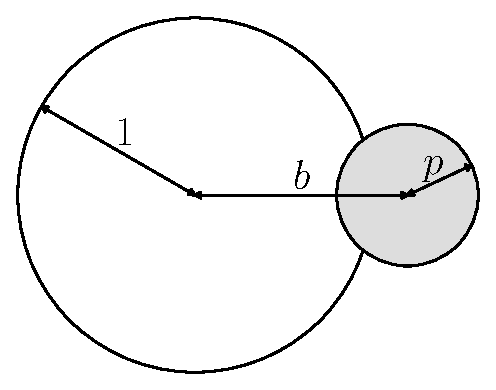
\includegraphics[width=\textwidth]{figures/geom.pdf}
    \end{center}
    \caption{Geometry of a transit. \figlabel{geom}}
\end{figure}



\end{document}
